\documentclass[11pt]{article}
\usepackage{amsmath,amssymb,amsthm}

\DeclareMathOperator*{\E}{\mathbb{E}}
\let\Pr\relax
\DeclareMathOperator*{\Pr}{\mathbb{P}}

\newcommand{\eps}{\varepsilon}
\newcommand{\inprod}[1]{\left\langle #1 \right\rangle}
\newcommand{\R}{\mathbb{R}}
\usepackage{graphicx}
\newcommand{\handout}[5]{
  \noindent
  \begin{center}
  \framebox{
    \vbox{
      \hbox to 5.78in { {\bf CS 224: Advanced Algorithms } \hfill #2 }
      \vspace{4mm}
      \hbox to 5.78in { {\Large \hfill #5  \hfill} }
      \vspace{2mm}
      \hbox to 5.78in { {\em #3 \hfill #4} }
    }
  }
  \end{center}
  \vspace*{4mm}
}

\newcommand{\lecture}[4]{\handout{#1}{#2}{#3}{Scribe: #4}{Lecture #1}}

\newtheorem{theorem}{Theorem}
\newtheorem{corollary}[theorem]{Corollary}
\newtheorem{lemma}[theorem]{Lemma}
\newtheorem{observation}[theorem]{Observation}
\newtheorem{proposition}[theorem]{Proposition}
\newtheorem{definition}[theorem]{Definition}
\newtheorem{claim}[theorem]{Claim}
\newtheorem{fact}[theorem]{Fact}
\newtheorem{assumption}[theorem]{Assumption}

% 1-inch margins, from fullpage.sty by H.Partl, Version 2, Dec. 15, 1988.
\topmargin 0pt
\advance \topmargin by -\headheight
\advance \topmargin by -\headsep
\textheight 8.9in
\oddsidemargin 0pt
\evensidemargin \oddsidemargin
\marginparwidth 0.5in
\textwidth 6.5in

\parindent 0in
\parskip 1.5ex

\begin{document}

\lecture{6 --- September 18, 2014}{Fall 2014}{Prof.\ Jelani Nelson}{Eric Balkanski}

\section{Overview}

We start a new topic, amortized analysis. In this lecture, we will explain what amortization is and apply it to the analysis of two data structures: Binomial Heaps and Fibonacci Heaps. 

\section{Amortization}

\subsection{Definition}
Suppose our data structure supports operations A, B, C. We say that the "amortized costs" of these operations are $t_a, t_b, t_c$ if any sequence of $n_a$ A operations, $n_b$ B operations, and $n_c$ $C$ operations takes time at most $ n_a t_a + n_b t_b + n_c t_c$.

\subsubsection{Potential functions}
A common way to prove amortized bounds is via the \textbf{potential function method}:

\begin{itemize}

\item Define potential $\Phi : \{$state of data structure$\} \rightarrow \mathbb{R}_{\geq 0}$

\item $\Phi$(empty structure) $> 0$

\item We perform $k$ operation with actual times $t_1,  \dots, t_k$ and that the states are $S_0, S_1, \dots, S_k$. The amortized cost of an operation $i$ is defined to be: $$t_i + \Phi(S_i) - \Phi(S_{i-1})$$

\item So the total amortized cost is bounded by $\sum_i (t_i + \Delta \Phi(i)) = \sum_i t_i + \Phi(S_k) \geq \sum_{t_i}$. 
\end{itemize}

Therefore, the common way to compute an amortized cost is to compute the worst 
$t_i + \Phi(S_i) - \Phi(S_{i-1})$ at any step.

\subsection{Example: Heaps}

Heaps are a data structure $H$ which support:
\begin{itemize}
\item insert(x) (the values $x$ are comparable)
\item deleteMin(): returns the min $x \in H$ then deletes it.
\item decreaseKey(p, k): replaces key at item $p$ with $k$ which must be at most p's current key.
\end{itemize}

Dijkstra's algorithm, which uses heaps, has a runtime $O(n (t_{insert} + t_{deleteMin}) + m t_{decreaseKey})$.

The existing implementations of heaps are the following:
\begin{itemize}
 \item Binary Heaps, by Williams \cite{heap}, which achieve $O(\lg n)$ worst case for
$ t_{insert}, t_{deleteMin}$, and  $t_{decreaseKey}$.
 
 \item Binomial Heaps, by Vuillemin \cite{bheap}, which achieve $O(1)$
 amortized cost for $t_{insert}$ and $O(\lg n)$ worst-case for $t_{deleteMin}$ and $t_{decreaseKey}$
 
 \item Fibonacci Heaps, by Fredman and Tarjan \cite{fheap}, which achieve $O(1)$ amortized cost for $t_{insert}$ and $t_{decreaseKey}$ and  $O(\lg n)$ amortized cost for $t_{deleteMin}$.
 \end{itemize}
 
 In this lecture, we will not cover binary heaps because they are not relevant to the Fibonacci Heaps. We will cover Binomial Heaps, since Fibonacci Heaps are a more optimal version of Binomial Heaps. Related work also include:
 
 \begin{itemize}
 
 \item Kaplan, Tarjan and Zwickl \cite{kaplan} constructed heaps so that there is only one tree and not a forest.
 
 \item Brodal \cite{brodal} obtained the same bounds as Fibonacci Heaps but in worst case instead of in amortized cost. His solution has been described as complicated, and uses extendable arrays.
 
 \item  Brodal, Lagogiannis, Tarjan \cite{brodal2} obtained the same bounds in worst case in the pointer machine model.

\end{itemize}

We note that we cannot improve the bound of $O(\lg n)$ for $t_{deleteMin}$ in the comparison model while keeping other operations constant time, since otherwise we would be able to sort in $o(n \lg n)$ time, which is impossible.

\section{Binomial Heaps}

\subsection{Definition}
In binomial heaps, each item is a node. We maintain these nodes in a forest as follow:

\begin{itemize}
\item If $x$ is the parent of $y$, then $key(x) \leq key(y)$.
\item For a tree in our heap, its "rank" is the degree of its root.
\item A tree with rank $k$ has $2^k$ nodes in it
\item For each $k$, we will have at most 1 tree of rank $k$.
\item Roots of trees of rank $k$ have $k$ subtrees, these are trees of ranks $0,1,\dots, k-1$.
\end{itemize}

\begin{figure}
\centering
\scalebox{0.6}{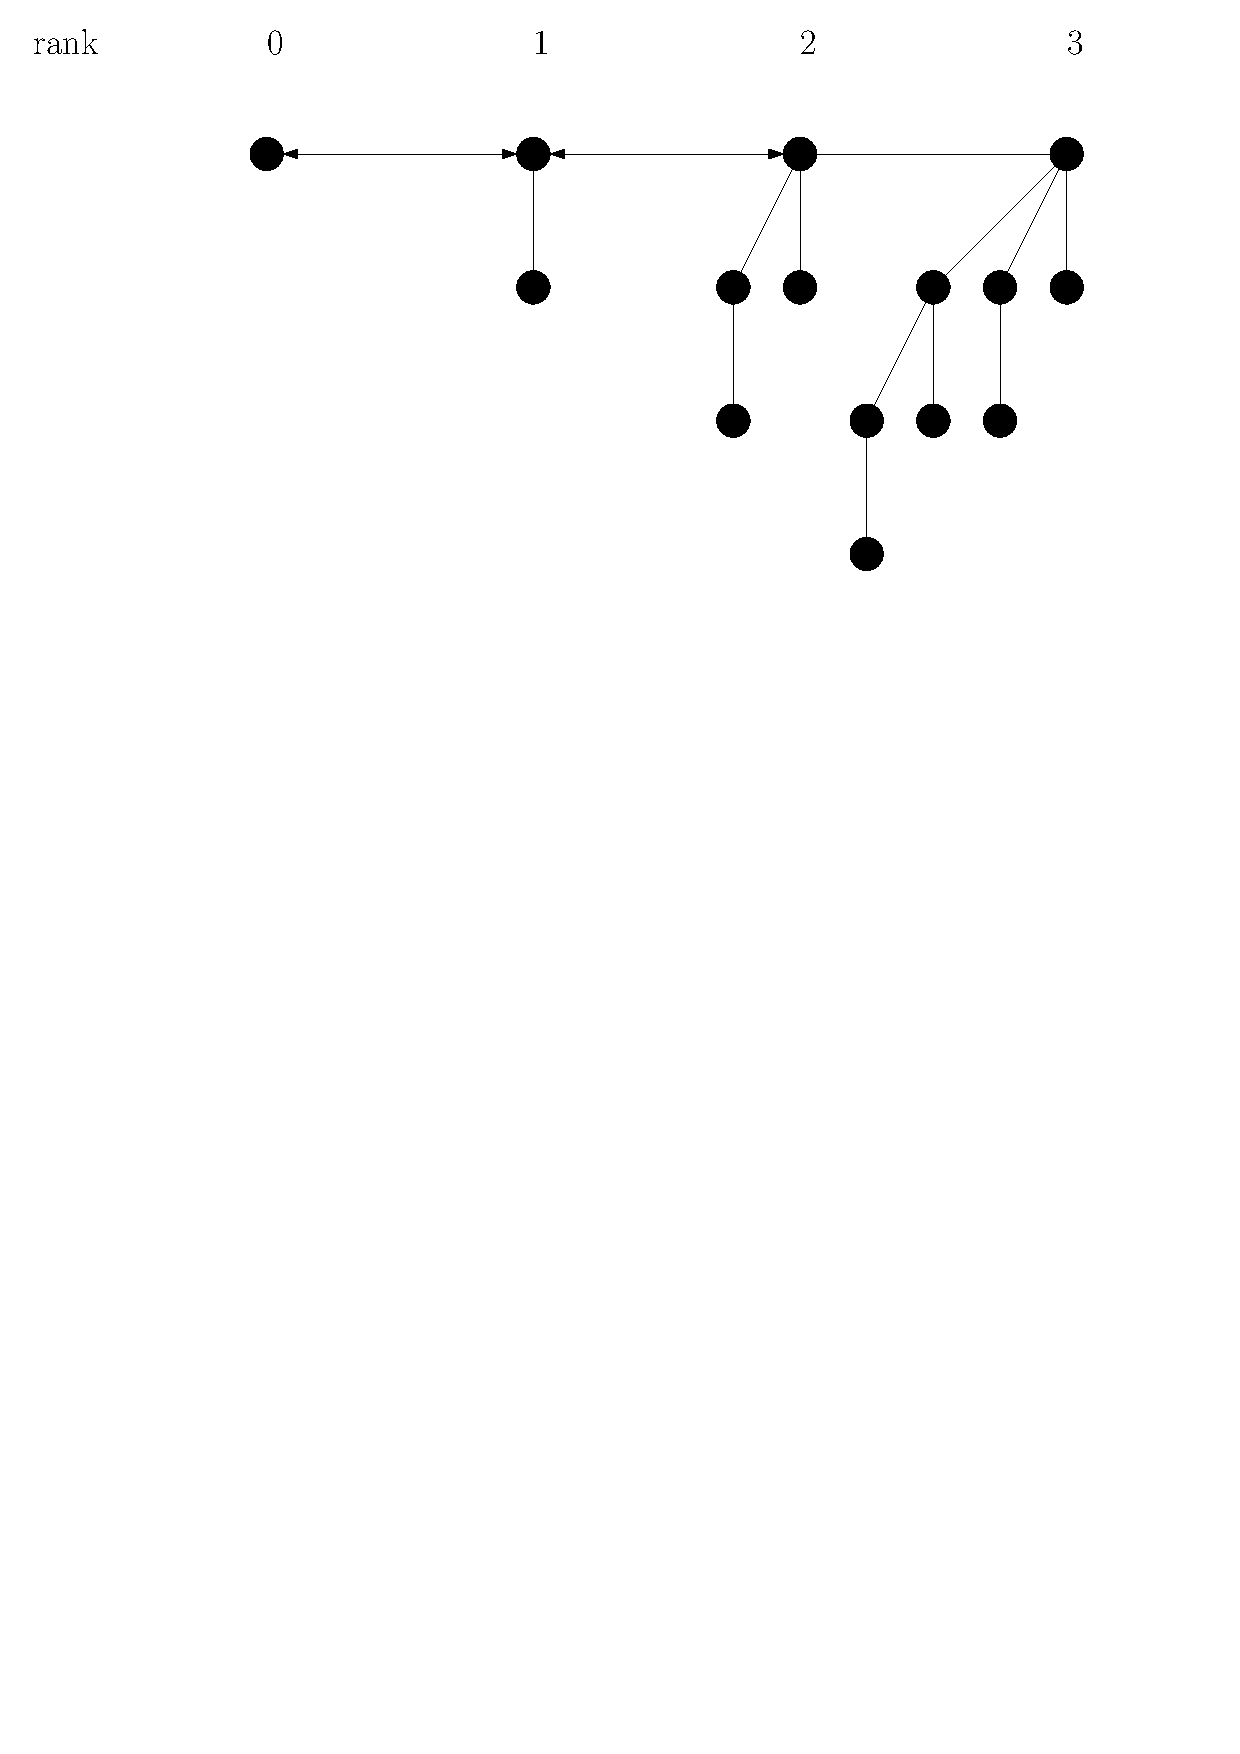
\includegraphics{binheap}}
\caption{A binomial heap with trees of rank 0, 1, 2, and 3.}
\end{figure}

The roots of the trees are kept in a linked list, as shown in Figure 1.

\subsection{Operations on Binomial Heaps}

\begin{itemize}
\item decreaseKey: Change the key, then keep swapping upward until we satisfy the property of parents having lower keys than children.

\item insert(x): Add a new singleton tree to forest, then repeatedly merge trees of equal rank until we have trees that are all of different ranks. This can be seen as a binary addition: for example, if we have trees of rank 4,2, and 1 and we had a singleton, then 1011 + 0001 = 1100. So we then have trees of rank 4 and 3.

\item deleteMin Remove root of some tree, insert all its children as roots in the main forest. Now merge trees of equal rank the same way as we did in insert(x).
\end{itemize}

\subsection{Worst Case Analysis}
In the worst case, all operations take $\Theta(\lg n)$ time. In the case of decreaseKey, we could decrease  a leaf in the tree of highest rank and have to swap until the root. Since the biggest tree has height $\Theta(\lg n)$, this would take $\Theta(\lg n)$ time in the worst case. In the case of insert and deleteMin, we could have trees of rank 1, 2, \dots, $m$. We would then have to repeatedly merge $\Theta(\lg n)$ times to get a tree of rank $m+1$. 

\subsection{Amortized analysis}
We now study the amortized cost and let the potential function be $\Phi$(data structure state) = number of trees. Let $T$ be the number of trees before an insertion and $t$ be the number of trees after an insertion. The actual costs of insertions are $O(T - t + 1)$. Therefore, the
amortized cost of insertion is: actual cost + $\Delta \Phi = T - t + 1 + t - T = 1$

\section{Fibonacci Heaps}

\subsection{The structure}
The main idea in Fibonacci Heaps is to be lazy. We do not want to do work until we really need to. In the case of Binomial Heaps, there is no reason for insertions to spend time consolidating the trees to maintain the Heap structure, deleteMin can do that. So when we insert an element, we just create a singleton and add it to the structure without doing any merges.
 
The problem could now come from decreaseKey, in the case where we repeatedly decrease keys that are leaves of a large tree. A really lazy possible decreaseKey is to decrease $x$'s key, and if $x$ is now smaller than parent, then cut $x$'s tree out and place as a top level tree.The problem with this approach is that we could have a tree of rank $k$, with many decreaseKey on the nodes that are neither the root nor a child of root, which would give us a tree of rank $k$ with $k+ 1$ leaves.

The fix is as follows. If node $p$ loses one child $x$ due to decreaseKey, then no problem. If $p$ loses a second child, we cut $p$ out of its tree and make $p$'s tree a top level tree. With this fix in hand, it is possible to prove Lemma~\ref{lem:fib} below.

\begin{definition}
We define the {\em Fibonacci numbers} $\{F_k\}_{i=0}^\infty$ via the recurrence
$$
F_k =
\begin{cases}
0,\ \text{ if } k=0\\
1,\ \text{ if } k = 1\\
F_{k-1} + F_{k-2},\ \text{otherwise}
\end{cases}
$$
\end{definition}

\begin{lemma}\label{lem:fib}
A tree in a Fibonacci heap with rank $k$ has at least $F_{k+2}$ nodes.
\end{lemma}

\subsection{Amortized Analysis}
We claim that  $t_{insertion}, t_{decreaseKey} = O(1)$ and that $t_{decreaseMin} = O(\lg n)$.

\begin{proof}
Define $mark(x) = \begin{cases} 1& \mbox{if x has lost child} \\
 0 & \mbox{else}
  \end{cases}
 $ 
 
 and the potential function to be 

$\Phi(state) = \mbox{\# trees} + 2 (\mbox{\# marked items}) = T(H) + 2 M(H)$

\begin{itemize}

\item Insertion. actual cost + $\Delta \Phi$ = O(1) + 1 = O(1)

\item deleteMin. $T + \Delta T(H) + 2\Delta M(H) \leq T + t- T + 0 = O(t)$ where $t$ is the number of trees left after consolidation, and $T$ is before consolidation. That is, we keep merging trees of equal rank until for each rank $k$, at most one tree of rank $k$ exists in our data structure. Now note that a rank $k$ tree has at least $F_{k+2} \ge \sqrt{2}^k$ nodes. Therefore the largest rank of any tree in our data structure can be at most $\log_{\sqrt{2}} n$ (since there are only $n$ nodes in the entire forest), implying $t \le (\log_{\sqrt{2}} n) + 1 = O(\log n)$.

\item decreaseKey. We have two cases.
\begin{itemize} 
\item Case 1: $x$ does not get cut out.

actual cost + $\Delta \Phi = O(1) + 0 = O(1)$.

\item Case 2: We do some number $c > 0$ of cascaded cuts ($c$ levels of consecutive cuts). 

actual cost $+ \Delta T(H) + 2 \Delta M(H) \leq 
           c     +             c          +  ( - 2c + 2) = O(1)$
\end{itemize}
\end{itemize}

\end{proof}


Next time, we will study Splay trees, which has amortized cost $O(\lg n)$ for all operations. The benefit of Splay trees is that they have very nice properties, such as static optimality. Static optimality takes into account the frequency of searches of items in order to minimize the total cost of all operations.




\bibliographystyle{alpha}

\begin{thebibliography}{42}

\bibitem{heap}
John W. J.~Williams.
\newblock Algorithm 232: Heapsort.
\newblock {\em CACM 7}, 347--348, 1964.

\bibitem{bheap}
Jean~Vuillemin.
\newblock A Data Structure for Manipulating Priority Queues.
\newblock {\em CACM 21}, 309--314, 1978.

\bibitem{fheap}
Michael L.~Fredman, Robert E.~Tarjan.
\newblock  Fibonacci heaps and their uses in improved network optimization algorithms.
\newblock {\em JACM 34}, 596--615, 1987.

\bibitem{kaplan}
Haim~Kaplan, Robert E.~Tarjan, Uri~Zwickl.
\newblock  Fibonacci Heaps Revisited
\newblock {\em arXiv}, 1407.5750, 2014.

\bibitem{brodal}
Gerth S.~Br{\o}dal.
\newblock  Worst-case efficient priority queues.
\newblock {\em SODA}, 52--58, 1996.

\bibitem{brodal2}
Gerth S.~Br{\o}dal, George~Lagogiannis, Robert E.~Tarjan.
\newblock  Strict Fibonacci Heaps
\newblock {\em STOC}, 1177-1184, 2012.

\end{thebibliography}

\end{document}